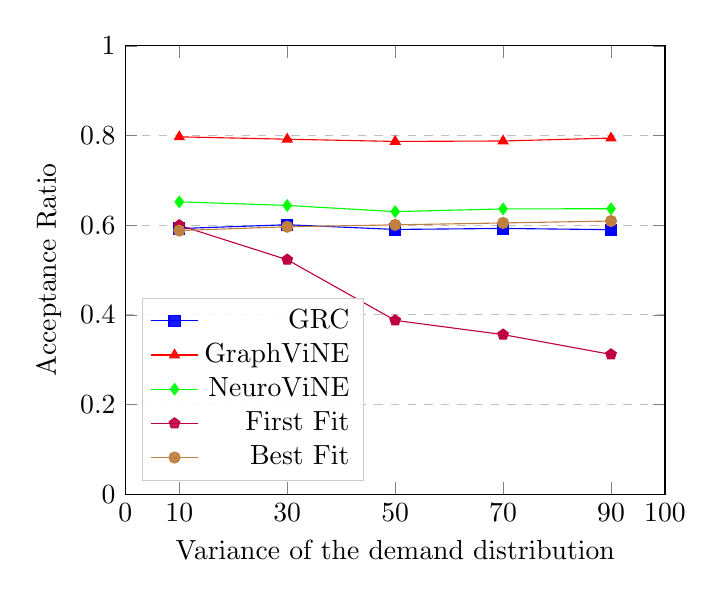
\begin{tikzpicture}
\begin{axis}[
    legend cell align={right},
    legend style={fill opacity=0.9, draw opacity=1, text opacity=1, draw=white!80!black},
    xlabel={Variance of the demand distribution},
    ylabel={Acceptance Ratio},
    xmin=0, xmax=100,
    ymin=0, ymax=1,
    xtick={0,10,30,50,70,90, 100},
    % ytick={0,100,200,300,400,500},
    legend pos=south west,
    ymajorgrids=true,
    grid style=dashed,
]

\addplot[
    color=blue,
    mark=square*,
    ]
    coordinates {
    (10,0.5923980995248812)
    (30,0.6009002250562641)
    (50,0.59039759939985)
    (70,0.5926481620405102)
    (90,0.5898974743685921)
    };
\addlegendentry{GRC}

\addplot[
    color=red,
    mark=triangle*,
    ]
    coordinates {
    (10,0.7969492373093273)
    (30,0.7916979244811203)
    (50,0.7866966741685422)
    (70,0.7876969242310577)
    (90,0.7941985496374093)
    };
\addlegendentry{GraphViNE}

\addplot[
    color=green,
    mark=diamond*,
    ]
    coordinates {
    (10,0.6519129782445612)
    (30,0.6439109777444361)
    (50,0.6301575393848462)
    (70,0.6361590397599399)
    (90,0.6366591647911978)
    };
\addlegendentry{NeuroViNE}

\addplot[
    color=purple,
    mark=pentagon*,
    ]
    coordinates {
(10,0.5996499124781196)
(30,0.5228807201800449)
(50,0.3875968992248062)
(70,0.35583895973993496)
(90,0.3115778944736184)
    };
\addlegendentry{First Fit}

\addplot[
    color=brown,
    mark=otimes*,
    ]
    coordinates {
(10,0.5878969742435609)
(30,0.5963990997749438)
(50,0.6006501625406351)
(70,0.6049012253063266)
(90,0.6091522880720179)
    };
\addlegendentry{Best Fit}





\end{axis}
\end{tikzpicture}